%Notes by Harsh Mistry 
%Math 239
%based on Template from : https://www.cs.cmu.edu/~ggordon/10725-F12/template.tex

\documentclass{article}
\setlength{\oddsidemargin}{0.25 in}
\setlength{\evensidemargin}{-0.25 in}
\setlength{\topmargin}{-0.6 in}
\setlength{\textwidth}{6.5 in}
\setlength{\textheight}{8.5 in}
\setlength{\headsep}{0.75 in}
\setlength{\parindent}{0 in}
\setlength{\parskip}{0.1 in}
\usepackage{amsfonts,graphicx, amssymb}
\usepackage[fleqn]{amsmath}
\usepackage{fixltx2e}
\usepackage{color}
\usepackage{tcolorbox}
\usepackage{lipsum}
\usepackage{listings}
\usepackage{scrextend}
\tcbuselibrary{skins,breakable}
\usetikzlibrary{shadings,shadows}
\usepackage{graphicx}
\graphicspath{ {images/} }
\newcounter{lecnum}
\renewcommand{\thepage}{\thelecnum-\arabic{page}}
\renewcommand{\thesection}{\thelecnum.\arabic{section}}
\renewcommand{\theequation}{\thelecnum.\arabic{equation}}
\renewcommand{\thefigure}{\thelecnum.\arabic{figure}}
\renewcommand{\thetable}{\thelecnum.\arabic{table}}
\newcommand{\lecture}[4]{
   \pagestyle{myheadings}
   \thispagestyle{plain}
   \newpage
   \setcounter{lecnum}{#1}
   \setcounter{page}{1}
   
   
%Info Box 
   \begin{center}
   \framebox{
      \vbox{\vspace{2mm}
    \hbox to 6.28in { {\bf Math 239 - Introduction to Combinatorics
	\hfill Spring 2017} }
       \vspace{4mm}
       \hbox to 6.28in { {\Large \hfill Lecture #1: #2  \hfill} }
       \vspace{2mm}
       \hbox to 6.28in { {\it Lecturer: #3 \hfill Notes By: #4} }
      \vspace{2mm}}
   }
   \end{center}
   
   \markboth{Lecture #1: #2}{Lecture #1: #2}



 
}

\renewcommand{\cite}[1]{[#1]}
\def\beginrefs{\begin{list}%
        {[\arabic{equation}]}{\usecounter{equation}
         \setlength{\leftmargin}{2.0truecm}\setlength{\labelsep}{0.4truecm}%
         \setlength{\labelwidth}{1.6truecm}}}
\def\endrefs{\end{list}}
\def\bibentry#1{\item[\hbox{[#1]}]}

\newcommand{\fig}[3]{
			\vspace{#2}
			\begin{center}
			Figure \thelecnum.#1:~#3
			\end{center}
	}
	
	\newcommand{\bs}{
		\texttt{\char`\\ \hspace{0.1cm}} 
	}
	

	
\newcommand{\pipe}{\(\mid\)}
\newcommand{\ctr}{\(\wedge\)}

\newtheorem{theorem}{Theorem}[lecnum]
\newtheorem{lemma}[theorem]{Lemma}
\newtheorem{ex}[theorem]{Example}
\newtheorem{expx}[theorem]{Problem}
\newtheorem{prop}[theorem]{Proposition}
\newtheorem{claim}[theorem]{Claim}
\newtheorem{corollary}[theorem]{Corollary}
\newtheorem{definition}[theorem]{Definition}
\newenvironment{proof}{{\bf Proof:}}{\hfill\rule{2mm}{2mm}}
\newcommand\E{\mathbb{E}}

%color definitions :
\definecolor{darkred}{rgb}{0.55, 0.0, 0.0}
\definecolor{lightcoral}{rgb}{0.94, 0.5, 0.5}
\definecolor{tomato}{rgb}{1.0, 0.39, 0.28}
\definecolor{lightgray}{rgb}{.9,.9,.9}
\definecolor{darkgray}{rgb}{.4,.4,.4}
\definecolor{purple}{rgb}{0.65, 0.12, 0.82}
\definecolor{lightgreen}{rgb}{0.56, 0.93, 0.56}
\definecolor{darkgreen}{rgb}{0.0, 0.2, 0.13}
\definecolor{limegreen}{rgb}{0.2, 0.8, 0.2}
\definecolor{lightblue}{rgb}{0.68, 0.85, 0.9}
\definecolor{darkblue}{rgb}{0.0, 0.0, 0.55}


%Environments
\newenvironment{exblock}[1]{%
    \tcolorbox[beamer,%
    noparskip,breakable,
    colback=lightgreen,colframe=darkgreen,%
    colbacklower=limegreen!75!lightgreen,%
    title=#1]}%
    {\endtcolorbox}

\newenvironment{ablock}[1]{%
    \tcolorbox[beamer,%
    noparskip,breakable,
    colback=lightcoral,colframe=darkred,%
    colbacklower=tomato!75!lightcoral,%
    title=#1]}%
    {\endtcolorbox}

\newenvironment{cblock}[1]{%
    \tcolorbox[beamer,%
    noparskip,breakable,
    colback=lightblue,colframe=darkblue,%
    colbacklower=darkblue!75!lightblue,%
    title=#1]}%
    {\endtcolorbox}


%Languages
\lstdefinelanguage{JavaScript}{
  keywords={typeof, new, true, false, catch, function, return, null, catch, switch, var, if, in, while, do, else, case, break},
  keywordstyle=\color{blue}\bfseries,
  ndkeywords={class, export, boolean, throw, implements, import, this},
  ndkeywordstyle=\color{darkgray}\bfseries,
  identifierstyle=\color{black},
  sensitive=false,
  comment=[l]{//},
  morecomment=[s]{/*}{*/},
  commentstyle=\color{purple}\ttfamily,
  stringstyle=\color{red}\ttfamily,
  morestring=[b]',
  morestring=[b]"
}

%Listings
\lstset{
   language=JavaScript,
   backgroundcolor=\color{lightgray},
   extendedchars=true,
   basicstyle=\footnotesize\ttfamily,
   showstringspaces=false,
   showspaces=false,
   numbers=left,
   numberstyle=\footnotesize,
   numbersep=9pt,
   tabsize=2,
   breaklines=true,
   showtabs=false,
   captionpos=b
}


%Start
\begin{document}

\lecture{24}{June 24th, 2017}{Alan Arroyo Guevara}{Harsh Mistry}
\begin{center}
\textcolor{red}{Missed This Lecture, Notes Taken By Xyan Bhatnagar}
\end{center}
\begin{theorem}
If T is a spanning tree of G and \(e \in E(G) \bs E(T) \) then T + e has a unique cycle c. Moreover for every \(e^\prime \in E(C) \bs \{e\}, T^\prime : = (T + e) - e^\prime \) is a spanning tree 
\end{theorem}

\textbf{Notation : \(T + e = (V(T), E(T) \cup \{e\})\)}

\begin{proof}
Let e = xy and Let P be a unique xy-path in T.\\ As every cycle in \(T + e\) contains e. 
\(C = P + e\) is the unique cycle in \(T + e\) \\
\newline 
Let \(e^\prime \in E(P) \subseteq E(C)\). As \(e^\prime\) is not a bridge in \(T + e\). Then \(T^\prime = (T+e) - e^\prime \) is connected 
$$ \mid E(T^\prime) \mid = \mid E(T) \mid = \mid V(T) \mid - 1 = \mid V(T^\prime) \mid -1 $$
By previous theorem, \(T^\prime\) is a tree and \(\mid V(T^\prime) \mid = \mid V(T) \mid = \mid V(G) \mid.\) So it is a spanning tree 
\end{proof}

\section{Characterizing Bipartite Graphs}
\begin{center}
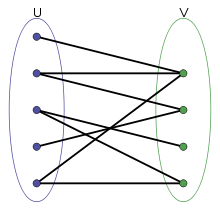
\includegraphics[scale=0.5]{12}
\end{center}
G is bipartite \(\iff\) V(G) can be coloured using 2 colours so that no 2 adjacent vertices have the same color

\begin{exblock}{Observations}
\begin{itemize}
\item A graph that contains a cycle of off length (odd cycle) as a sub graph is \textbf{not bipartite}.
\item Trees are bipartite
\end{itemize}
\end{exblock}

\begin{theorem}
A graph is bipartite if and only if it has no odd cycles as a sub-graph 
\end{theorem}
\newpage
\begin{proof}
\begin{itemize}
\item[\(\rightarrow\)] Use previous observations
\item[\(\leftarrow\)] Suppose G has no odd cycles. Assume that G is connect (or we treat components separately). \\
Let T be a spanning tree of G and Let \(A \cup V = V(T)\) be a bipartition of T. \\ \newline 
We claim that \(A \cup B\) is also a bipartition of G. Suppose not, then there exists \(e = uv \in E(G) \bs E(T)\) where u and v both belong to A or B. \\ \newline 
Let \(u,v \in A\) and Let P be the uv-path in T.\\
Length(P) is even because \(u,v \in A \implies p+e\) is an odd cycle. \textbf{Contradiction}  
\end{itemize}
\end{proof}

\section{Breadth-First Search Trees (BFS)}

\begin{definition}
A queue is an ordered list 
$$ Q : q_1, q_2, q_3, \ldots, q_n $$
where every new element added to Q is added at the end. The first element in Q is the \textbf{active element}
\end{definition}

\subsection*{BFS Algorithm}
\begin{itemize}
\item[\textbf{Input:}] Graph G and \(r \in V(G)\)
\item[\textbf{Output:}] Spanning Tree T or that G is not connected
\item[\textbf{Process:}]
\begin{enumerate}
\item Initialization \\
\(T = (\{r\}, \phi)\)  r = vertices and \(\phi\) = edges\\
\(P:V(G) \rightarrow V(G) \cup \{null\} \)\\
\(P(v) \rightarrow null \)\\
\(Q = r\)
\item Operations
\begin{lstlisting}
While Q != phi 
	Let u be the active vertex in Q
	While u has a neighbour not in V(T) 
		Add v and uv to T 
		Let P(v) = u
		Add v to Q 
	Remove u from Q
\end{lstlisting}
\item Output (T,P)
\end{enumerate}
\end{itemize}

\end{document} 